\documentclass[11pt]{article}
\usepackage[margin=0.8in]{geometry}
\usepackage{bm}
\usepackage{amsfonts}
\usepackage{amsthm}
\usepackage{amssymb}
\usepackage{amsmath}
\usepackage{xcolor}
\usepackage{tikz}
\usepackage[colorlinks = true]{hyperref}
\usepackage{mathtools}              
\usepackage{cellspace}            
\setlength\cellspacetoplimit{10pt}   
\setlength\cellspacebottomlimit{10pt}


\title{\textbf{Week 5 Discussion Question Solution}}
\author{UNSW Business School, ACTL3182}
\date{October 2020}

%Comment out for no section colours.
\usepackage{titlesec}
%\titleformat{\section}{\Large\sffamily\bfseries\color{red}}{\thesection}{0.5em}{}[]
%\titleformat{\subsection}{\color{red!75}\large\sffamily\bfseries}{\thesubsection}{0.5em}{}
%\titleformat{\subsubsection}{\color{red!50}\normalsize\sffamily\bfseries}{\thesubsubsection}{0.5em}{}

\begin{document}
	\maketitle
	
	\section*{1. Feedback}
		\subsection*{Done Well}
			\begin{itemize}
				\item Clearly all of you know how to apply the Binomial Model. Good understanding shown here.
				\item Most of you correctly priced the calls in part iii, even if you did not know how to do part ii.
			\end{itemize}
		\subsection*{Mistakes}
			\begin{itemize}
				\item The biggest mistake was in determining whether there was an arbitrage opportunity in part ii. There was a wide range of incorrect approaches including stating that it was not possible to determine whether there was arbitrage or relating the risk-free return to the stock returns without proper justification and calculation. \\\\
				The simplest approach observes that all risk-neutral probabilities are between 0 and 1 and that this is equivalent to an arbitrage-free market. This is two sentences of reasoning and no calculation is needed since the probabilities were calculated in part i. \\\\
				Alternatively, one can show that the up and down factors of the stock always satisfy
				$$d < e^{r} < u$$
				For example, for $t=1$, we have
				$$\frac{73.5}{70} < 1.1 < \frac{91}{70}$$
				and similarly for the two outcomes at $t=2$, so there is no arbitrage. For additional information see tutorial exercise 3.25 part 1, and as an exercise, prove this is equivalent to (i.e if and only if) $0<q<1$.
				\item You were given the \textbf{effective} per period risk-free rate in the bonds;
				\[	\frac{B(1)}{B(0)} = \frac{B(2)}{B(1)} = 1.1 = e^{r}
					\]
				This is \textbf{not} the continuously-compounded risk-free rate used in the Binomial Model; some of you mistakenly used $r=0.1$. The correct equation is $r = \ln(1.1)$, but you do not actually need to calculate $r$. Simply use the effective accumulation factor of $1.1$. For example $e^{-r} = 1.1^{-1}$.
				\item Some of you calculated $f_{1},f_{2},f_{3}$ but did not match these to the call prices of each market scenario.
			\end{itemize}
		\subsection*{Concept Tips}
			\begin{itemize}
				\item Use tables to simplify the layout of your final answers. Tables were especially appropriate for this question since there were corresponding quantities for each scenario.
				\item Check that the total probability of all four scenarios adds to 1.
			\end{itemize}
		%\subsection*{Software Tips}
	\section*{2. Solution}
	Let $q_{i}$ for $i=1,2,3$ be the risk-neutral probabilities of the stock moving up in price at the corresponding nodes according to the trees below:
	\begin{center}
		\resizebox{5cm}{5.5cm}{
			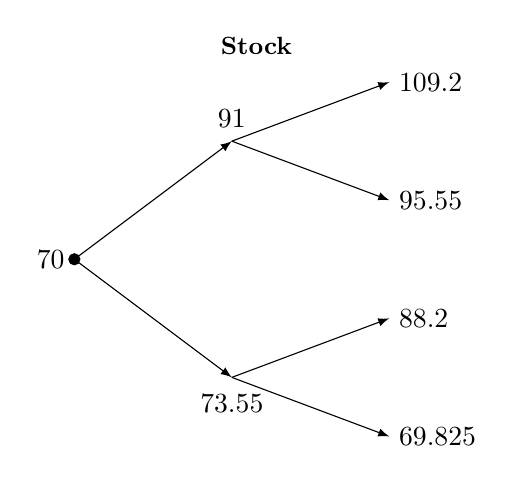
\begin{tikzpicture}
			%\tikzstyle{every node}=[font=\small];
			
			%Title
			%\node[above, font = \small\bfseries] at (current bounding box.north) {Stock};
			
			%Level 1
			\filldraw[fill=black] (0, 0) circle(2pt);
			\node[left] at (0, 0) {\( 70 \)};
			
			%Lines
			\draw[-latex] (0, 0) -- (2, 1.5);
			\draw[-latex] (0, 0) -- (2, -1.5);
			
			%Level 2
			\node[above] at (2, 1.55) {\( 91 \)};
			\node[below] at (2, -1.6) { \( 73.55 \)};
			
			%Lines
			\draw[-latex] (2, 1.5) -- (4, 2.25);
			\draw[-latex] (2, 1.5) -- (4, 0.75);
			\draw[-latex] (2, -1.5) -- (4, -0.75);
			\draw[-latex] (2, -1.5) -- (4, -2.25);
			
			%Level 3
			\node[right] at (4, 2.25) {\( 109.2 \)};
			\node[right] at (4, 0.75) {\( 95.55 \)};
			\node[right] at (4, -0.75) {\( 88.2 \)};
			\node[right] at (4, -2.25) {\( 69.825 \)};
			
			%Title
			\node[above, font = \small\bfseries] at (current bounding box.north) {Stock};
			\end{tikzpicture}
		}
		\hspace{2cm}
		\resizebox{5cm}{5.5cm}{
			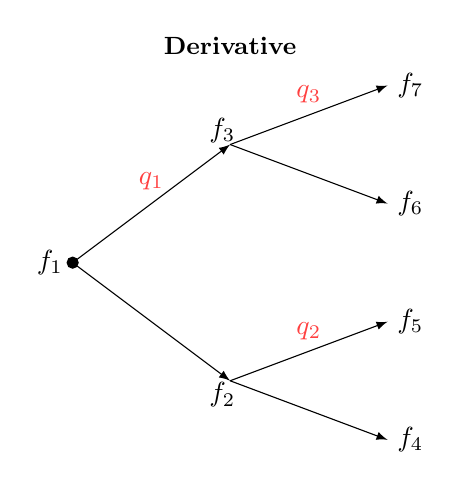
\begin{tikzpicture}
			%\tikzstyle{every node}=[font=\small];
			
			%Title
			%\node[above, font = \small\bfseries] at (current bounding box.north) {Stock};
			
			%Level 1
			\filldraw[fill=black] (0, 0) circle(2pt);
			\node[left] at (0, 0) {\( f_1 \)};
			
			%Lines
			\draw[-latex] (0, 0) -- (2, 1.5);
			\draw[-latex] (0, 0) -- (2, -1.5);
			
			%Level 2
			\node[above] at (1.9, 1.4) {\( f_3 \)};
			\node[below] at (1.9, -1.4) { \( f_2 \)};
			
			%Lines
			\draw[-latex] (2, 1.5) -- (4, 2.25);
			\draw[-latex] (2, 1.5) -- (4, 0.75);
			\draw[-latex] (2, -1.5) -- (4, -0.75);
			\draw[-latex] (2, -1.5) -- (4, -2.25);
			
			%Level 3
			\node[right] at (4, 2.25) {\( f_7 \)};
			\node[right] at (4, 0.75) {\( f_6 \)};
			\node[right] at (4, -0.75) {\( f_5 \)};
			\node[right] at (4, -2.25) {\( f_4 \)};
			
			%Risk Neutral probabilities.
			\node[red!75, above] at (1, 0.8) {\( q_1 \)};
			\node[red!75, above] at (3, -1.1) {\( q_2 \)};
			\node[red!75, above] at (3, 1.9) {\( q_3 \)};
			%Title
			\node[above, font = \small\bfseries] at (current bounding box.north) {Derivative};
			\end{tikzpicture}
		}
	\end{center}
	
	\noindent \textbf{i. } We first compute the risk-neutral probabilities at each node:
	\[	q_{j} = \frac{s_{\text{now}}e^{r\delta t} - s_{\text{down}}}{s_{\text{up}} - s_{\text{down}}},
		\]
	\begin{align*}
		q_{1} & = \frac{70(1.1) - 73.5}{91 - 73.5} = \frac{1}{5} \\[5pt]
		q_{2} & = \frac{73.5(1.1) - 69.825}{88.2 - 69.825} = \frac{3}{5}\\[5pt]
		q_{3} & = \frac{91(1.1) - 95.55}{109.2 - 95.55} = \frac{1}{3}\\
	\end{align*}
	The probability of each scenario is therefore given by:
	\begin{center}
		\begin{tabular}{cl}
			\textbf{Scenario} & \textbf{Probability}\\[5pt]
			\hline
			\hline
			&\\[-2ex]
			$\omega_{1}$ & $\displaystyle q_{1}q_{3} = \frac{1}{15}$\\[5pt]
			\hline
			&\\[-2ex]
			$\omega_{2}$ & $\displaystyle q_{1}(1-q_{3}) = \frac{2}{15}$\\[5pt]
			\hline
			&\\[-2ex]
			$\omega_{3}$ & $\displaystyle (1-q_{1})q_{2} = \frac{12}{25}$\\[5pt]
			\hline
			&\\[-2ex]
			$\omega_{4}$ & $\displaystyle (1-q_{1})(1-q_{2}) = \frac{8}{25}$\\[5pt]
			\hline
			\end{tabular}
		\end{center}
	\newpage
	\noindent \textbf{ii. } There is no arbitrage iff all the risk-neutral probabilities are between 0 and 1. 
	%(see tutorial question 3.25 part 1, then as a simple exercise prove this condition is equivalent to $0<q<1$). 
	Clearly $0<q_{i}<1$ for $i=1,2,3$, so there is no arbitrage in the market. \\\\
	
	\noindent \textbf{iii. } 
	The payoff of a European call option is $(S_{T} - K)_{+}$. Hence the payoff in each scenario is:
	\begin{center}
		\begin{tabular}{cl}
			\textbf{Scenario} & \textbf{    Payoff}\\
			\hline
			\hline
			$\omega_{1}$ & $(109.2 - 80)_{+} = 29.2$\\
			\hline
			$\omega_{2}$ & $(95.55 - 80)_{+} = 15.55$\\
			\hline
			$\omega_{3}$ & $(88.2 - 80)_{+} = 8.2$\\
			\hline
			$\omega_{4}$ & $(69.825 - 80)_{+} = 0$\\
			\hline
			\\
		\end{tabular}
	\end{center}
	Now, using $f_{\text{now}} = e^{-r}\cdot\mathbb{E}_{\mathcal{Q}}[f_{\text{next}}] = e^{-r}(q_{\text{now}}f_{\text{up}} +(1-q_{\text{now}})f_{\text{down}})$, \\
	\begin{align*}
		f_{3} & = 1.1^{-1}\left[29.2q_{3} + 15.55(1 - q_{3})\right] = 18.2727\\
		f_{2} & = 1.1^{-1}\left[8.2q_{2} + 0(1-q_{2})\right] = 4.4727\\
		f_{1} & = 1.1^{-1}\left[q_{1}f_{3} + (1 - q_{1})f_{2}\right] = 6.5752\\
		\end{align*} 
	Under the risk-neutral measure $\bm{\mathcal{Q}}$, the price of any asset is equal to the expected payoff discounted at the risk-free rate. These are exactly the $f_{i}$'s that have been calculated, so the call prices in each scenario are:
	\begin{center}
		\begin{tabular}{cccc}
			\textbf{Scenario}  & $\bm{C(0)}$ & $\bm{C(1)}$ & $\bm{C(2)}$ \\
			\hline
			\hline
			$\omega_{1}$ & $6.5752$ & $18.2727$  & $29.2$ \\
			\hline
			$\omega_{2}$ & $6.5752$ & $18.2727$  & $15.55$ \\
			\hline
			$\omega_{3}$ & $6.5752$ & $4.4727$  & $8.2$ \\
			\hline
			$\omega_{4}$ & $6.5752$ & $4.4727$  & $0$ \\
			\hline
			\\
			\end{tabular}
		\end{center}
	You do not need to provide the above justification about the risk-neutral price in the exam for this type of question; it is provided for your revision.
	\end{document}